%---------------------------------------------------------------------------
% Preface

%\chapter*{Vorwort}

%Bla bla \dots

 %\cleardoublepage

%---------------------------------------------------------------------------
% Table of contents

% \setcounter{tocdepth}{2}
% \tableofcontents

%\cleardoublepage

%---------------------------------------------------------------------------
% Abstract

%\chapter*{Zusammenfassung}
% \addcontentsline{toc}{chapter}{Zusammenfassung}

%Bla bla \dots

% \cleardoublepage

\chapter*{Preamble}
 \addcontentsline{toc}{chapter}{Preamble}


This is the manual for the (very simple, but still quite powerfull) Matlab tool \proneu.  The tool uses the MATLAB Symbolic Math Toolbox\footnote{http://www.mathworks.ch/products/symbolic/} to derive the analytical global kinematics and equations of motion based on projected Newton-Euler methods.  In \secref{sec:theory}, a short summary about the theory (kinematics and dynamics) is given in combination with an outline of the implementation in MATLAB. \\ 
\begin{figure}[H]
	\centering
		\subfigure[3-link robot arm]{\includegraphics[height=3.5cm]{../RobotArmExample/robotArm3link_asm.pdf}}
		\subfigure[prismatic joint]{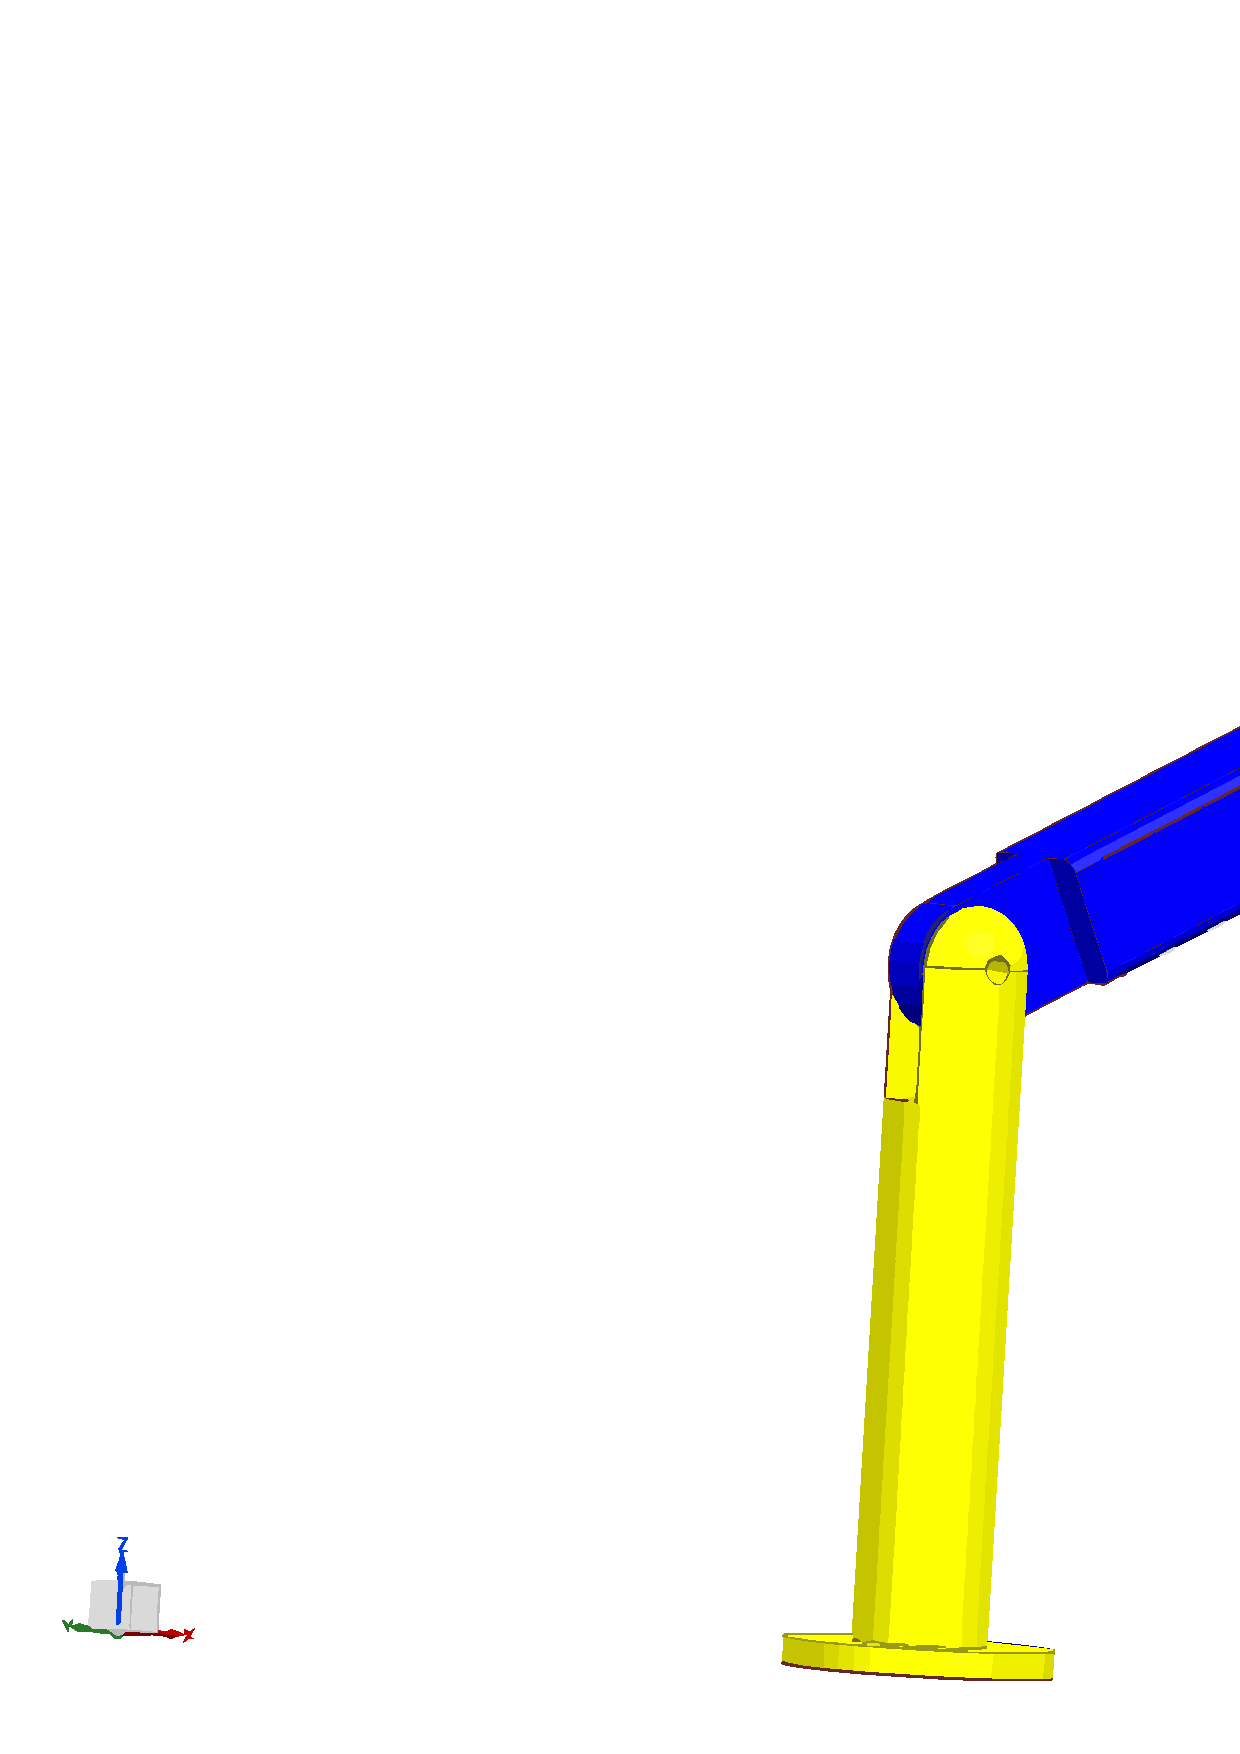
\includegraphics[height=3.5cm]{../RobotArmExample/robotArm_asm.pdf}}
		\subfigure[quadruped robot]{\includegraphics[height=3.5cm]{pics/3D_PR.pdf}}
	\caption{Three examples illustrating the use of this toolbox (\secref{sec:ex}).}
	\label{fig:exCol}
\end{figure}


Several examples (documented in \secref{sec:ex} as well as in the source files) highlight how this tool has to be used.  The user chooses the generalized coordinates, actuator and link parameters before setting up a very simple kinematic tree of the entire system.  The global kinematics and the equations of motion are symbolically derived and the user can visually check the robot configuration.  In the examples it is outlined, how the user can finally get function files, compiled mex-function, or C-code that can be used or embedded in any simulation environment.
\\

We intentionally kept this tool very simple for several reasons:  First, there exist (often commercially available) complex tools that are often a large overkill for most applications.  We do not want to have a sophisticated user front-end that allows adjusting everything without seeing behind the scenes, instead we appreciate tools where we can adapt everything for our needs.  In our specific case, we use this tool mostly for model based controllers, where we require to get the dynamics fast and efficiently in simulations or on the actual hardware.


\clearpage
% Version table
\begin{table}
\begin{tabular}[width=1\textwidth]{|p{2cm} p{10cm}|}
\hline
date: &Mar. 2012 \\
authors: &Christian Gehring \\
version: & 1.1 \\
info:    & minor fixes and improvements of the documentation, changed color of coordinate systems and added a world frame to plotBodies() \\
\hline
date: &Dec. 2011 \\
authors: &Marco Hutter \\
         &Christian Gehring \\
version: & 1.0 \\
info:    & First appearance of \proneu\\
\hline
\end{tabular}
\label{tab:version}
\caption{Revisions}
\end{table}


% software content table

\begin{table}
\begin{tabular}[width=1\textwidth]{|p{6cm} p{7cm}|}
\hline
\footnotesize \bf{utils/} &\footnotesize utility folder\\
\footnotesize.../computePNE.m & \footnotesize core file for global dynamics and projected Newton-Euler equations\\
\footnotesize.../dMATdt.m & \footnotesize full differentiation \\
\footnotesize.../eulerToRotMat$\_$A$\_$IB.m &\footnotesize rotation matrix from B to I frame, x-y-z definition \\
\footnotesize.../eulerToRotMat$\_$A$\_$BI.m &\footnotesize rotation matrix from I to B frame, x-y-z definition \\
\footnotesize.../plotBodies.m &\footnotesize visualization of (global) kinematic tree \\
\footnotesize.../skew.m &\footnotesize get skewing a matrix from vector \\
\footnotesize.../unskew.m &\footnotesize skew matrix to vector \\
\hline
\footnotesize\bf{examples/} &\footnotesize example folder\\
\footnotesize.../QuadrupedFreeFloat/genEoM.m &\footnotesize free floating quadruped Starl\textit{ETH} \\
\footnotesize.../RA3Link/genEoM.m &\footnotesize robot arm with 3 links and 3 revolute joints\\
\footnotesize.../RA3LinkPrismatic/genEoM.m &\footnotesize robot arm with 3 links and 1 prismatic joint \\
\footnotesize.../GenerateCode/createFunctionFiles.m &\footnotesize generating matlab and functions \\
\footnotesize.../GenerateCode/genCCodeMatrix.m &\footnotesize generate c-code of marix function \\
\footnotesize.../GenerateCode/genCCodeVariables.m &\footnotesize define parameters for c-code \\
\footnotesize.../GenerateCode/genCCodeExampleFile.m &\footnotesize example for c-code \\
\hline
\end{tabular}
\label{tab:content}
\caption{Software file content}
\end{table}
\normalsize
 \cleardoublepage

%---------------------------------------------------------------------------

% Table of contents

 \setcounter{tocdepth}{2}
 \tableofcontents
 
 \cleardoublepage